% =============================================================================
% DISCOVA: Discovering Inter-Domain Structural Holes via Stratified LLM
%          Distillation and Analogical Link Prediction
% ACL 2023 Style — Final Project Report
% =============================================================================
% COMPILATION INSTRUCTIONS:
%   pdflatex main.tex
%   bibtex main
%   pdflatex main.tex
%   pdflatex main.tex
%
% Or upload the entire /report folder to Overleaf as a new project.
% =============================================================================

\documentclass[11pt]{article}
\usepackage[hyperref]{acl2023}
% acl_natbib is a .bst bibliography style, not a package — do not \usepackage it

% Additional packages
\usepackage{times}
\usepackage{latexsym}
\usepackage[T1]{fontenc}
\usepackage[utf8]{inputenc}
\usepackage{microtype}
\usepackage{inconsolata}
\usepackage{booktabs}
\usepackage{multirow}
\usepackage{graphicx}
\usepackage{amsmath}
\usepackage{amssymb}
\usepackage{xcolor}
\usepackage{tikz}
\usepackage{pgfplots}
\pgfplotsset{compat=1.18}
\usepackage{algorithm}
\usepackage{algpseudocode}
\usepackage{subcaption}
\usepackage{enumitem}
\usepackage{url}
\usepackage{adjustbox}
\usepackage{colortbl}
\usepackage{tabularx}
\usepackage{array}
\usepackage{float}

\usetikzlibrary{shapes.geometric, arrows.meta, positioning, fit,
                backgrounds, calc, decorations.pathreplacing}

% Colour palette
\definecolor{funnel1}{RGB}{70,130,180}
\definecolor{funnel2}{RGB}{60,179,113}
\definecolor{funnel3}{RGB}{255,140,0}
\definecolor{highlight}{RGB}{200,50,47}
\definecolor{lightblue}{RGB}{219,234,254}
\definecolor{lightgreen}{RGB}{220,252,231}
\definecolor{lightorange}{RGB}{255,237,213}
\definecolor{darkblue}{rgb}{0,0,0.6}
\definecolor{darkgreen}{rgb}{0,0.4,0}

\hypersetup{
  colorlinks=true, linkcolor=darkblue,
  citecolor=darkgreen, urlcolor=darkblue
}

% Tighter list spacing
\setlist[itemize]{itemsep=2pt, topsep=3pt, parsep=0pt}
\setlist[enumerate]{itemsep=2pt, topsep=3pt, parsep=0pt}

% --------------------------------------------------------------------------
\title{Discovering Inter-Domain Structural Holes via Stratified LLM\\
Distillation and Analogical Link Prediction}

\author{
  Abhi Kommuri \quad Pranavi Sowreddy \quad Pavan Reddy \\
  Department of Computer Science and Engineering \\
  \texttt{\{abhireddy, pranavi, pavanreddy\}@institution.edu}
}
% --------------------------------------------------------------------------

\begin{document}
\maketitle

% =============================================================================
\begin{abstract}
% =============================================================================
Scientific breakthroughs frequently arise from transplanting a mature
algorithm from one domain to solve an analogous unsolved problem in another.
We present \textbf{DISCOVA} (Discovery of Inter-domain Structural COnnections
Via Analogical link prediction), a training-free six-stage pipeline over the
OGBN-ArXiv corpus (169,343 CS papers, 40 domains, 1.16M citation edges) that
automatically identifies such \emph{cross-domain structural holes}:\ pairs of
papers employing structurally identical algorithms that do not cite each other.
The core challenge is \emph{Domain Vocabulary Bias}: standard NLP embeddings
are dominated by domain-specific nouns, hiding shared algorithmic structure.
We overcome this via LLM-based domain normalization---replacing domain nouns
with neutral algebraic placeholders (``Parameter X,'' ``System Y'')---followed
by sentence-transformer cosine matching, citation-chasm filtering, and spaCy
dependency-tree structural verification.
The pipeline generates 5 ranked research hypotheses, each grounded in three
independent signals: embedding similarity ($\geq$0.90), Jaccard verb-set
structural overlap, and OGBN citation-graph neighborhood analysis.
Automated LLM scoring assigns a mean quality of 4.12/5.0 across five
scientific dimensions (Novelty, Significance, Effectiveness, Clarity,
Feasibility). A 2$\times$2 ablation study reveals that the Stanford Stanza
parser discovers 14\% more unique cross-domain types than spaCy, while
label-stratified Stage~1 sampling degrades end-to-end performance due to an
overly restrictive density floor.
Code and outputs are available at
\url{https://github.com/pavanreddy2480/Bridging-Structural-Holes}.
\end{abstract}

% Switch to two-column layout for the body of the paper
\twocolumn
\setlength{\parskip}{4pt plus 1pt}

% =============================================================================
\section{Introduction}
% =============================================================================

The most transformative discoveries in science often occur at disciplinary
intersections. The Kalman Filter, developed for control systems, became
the navigational core of GPS satellites. Simulated Annealing, modeled on
thermodynamic cooling, solved combinatorial optimization problems. The
Transformer architecture, designed for natural language, became the
foundation of protein structure prediction. None of these transfers were
identified systematically---they happened by accident.

We ask: \textbf{can a computational system reliably identify which mature
algorithm from domain~$X$ has not yet been applied to the structurally
equivalent unsolved problem in domain~$Y$?}

The fundamental obstacle is \emph{Domain Vocabulary Bias}. A machine
learning paper on stochastic gradient descent and an epidemiology paper on
disease-spread minimization may employ identical iterative optimization
procedures, yet standard NLP representations push them to opposite ends of
embedding space due to domain-specific nouns (\textit{loss surface},
\textit{weight vector} vs.\ \textit{reproduction number},
\textit{contact matrix}) dominating both texts. Existing approaches fail:
raw keyword matching, citation-network proximity, and even full-text embeddings
all succumb to this bias.

DISCOVA solves this through a \emph{three-layer computational funnel}
applied to OGBN-ArXiv \citep{hu2020open}.
(1)~\textbf{TF-IDF verb-density filtering}: 169K papers~$\to$~2,000
method-dense candidates using a curated 70-verb algorithmic vocabulary.
(2)~\textbf{LLM domain normalization + semantic matching}: domain nouns
replaced by neutral algebraic placeholders, then cosine similarity + citation
chasm filter yields 50 cross-domain structural hole candidates.
(3)~\textbf{Structural verification + hypothesis synthesis}: spaCy dependency
tree Jaccard overlap over full methodology texts, OGBN graph neighborhood
analysis, and LLM hypothesis generation.

\textbf{Contributions:}
\begin{itemize}
\item A three-layer funnel reducing 169,343 papers to 5 verified
  cross-domain research hypotheses with no model fine-tuning;
\item LLM-as-domain-equalizer: a novel surgical prompting strategy that
  neutralizes vocabulary bias by reducing abstracts to algebraic logic strings;
\item A bidirectional citation-chasm filter guaranteeing novelty of all
  predicted connections;
\item A multi-signal verification protocol (embedding sim + structural
  overlap + graph analysis);
\item A 2$\times$2 ablation study with three paradox-corrected metrics.
\end{itemize}

% =============================================================================
\section{Related Work}
% =============================================================================

\paragraph{Automated Scientific Discovery.}
\citet{tshitoyan2019unsupervised} used word2vec on materials science abstracts
to predict future material discoveries, but their approach relies on
domain-specific co-occurrence patterns and cannot generalize across
disciplinary boundaries. \citet{hope2021extracting} extracted structured
research contributions for within-domain knowledge graphs.

\paragraph{Citation Network Link Prediction.}
\citet{wang2021science} analyzed citation dynamics to predict scientific
impact, but citation-based methods are structurally incapable of identifying
connections that no one has yet made \citep{zhang2018link}. Graph neural
network link prediction \citep{zhang2018link} predicts likely co-citation,
not missing bridges across distant domains.

\paragraph{Structural Holes.}
Burt's structural holes \citep{burt2004structural} in social networks
identify nodes bridging disconnected communities. We adapt this to citation
networks: a cross-domain structural hole is a high-similarity paper pair
with no citation path, representing an unexploited research bridge.

\paragraph{LLM for Knowledge Extraction.}
Chain-of-thought prompting \citep{wei2022chain} and recent LLM-based
information extraction show strong performance, but none use LLMs as
\emph{vocabulary-bias eliminators}. Our distillation approach---preserving
algorithmic verbs while stripping domain nouns---is a novel prompting paradigm.

% =============================================================================
\section{Dataset}
% =============================================================================

\subsection{OGBN-ArXiv}

We use the \texttt{ogbn-arxiv} benchmark \citep{hu2020open}, a directed
citation graph of CS papers on ArXiv. Table~\ref{tab:dataset} summarises
the key statistics.

\begin{table}[h]
\small
\centering
\begin{tabular}{lr}
\toprule
\textbf{Property} & \textbf{Value} \\
\midrule
Total nodes (papers) & 169,343 \\
Directed citation edges & 1,166,243 \\
Subject categories (labels) & 40 \\
Time span & 1991--2020 \\
Avg.\ degree & 6.88 \\
\midrule
Method-dense papers (Stage~1) & 2,000 \\
Cross-domain pairs (Stage~3) & 50 \\
Verified pairs (Stage~4) & 9 \\
Structural hole predictions (Stage~5) & 12 \\
Final hypotheses (Stage~6) & 5 \\
\bottomrule
\end{tabular}
\caption{OGBN-ArXiv statistics and pipeline funnel sizes.}
\label{tab:dataset}
\end{table}

\subsection{Stage 1 Domain Distribution}

The global TF-IDF filter produces a notably skewed selection:
\texttt{cs.MA} (499 papers, 24.9\%), \texttt{cs.GL} (443, 22.1\%),
and \texttt{cs.NE} (389, 19.4\%) together account for 66.6\% of the
top-2,000 (Gini coefficient 0.765). Three categories
(\texttt{cs.DM}, \texttt{cs.ET}, \texttt{cs.SC}) have zero papers
above the method-density threshold, reflecting a genuine absence of
procedural content in those domains rather than a sampling artifact.

% =============================================================================
\section{Methodology}
% =============================================================================

\subsection{Pipeline Architecture}

Figure~\ref{fig:pipeline} depicts the DISCOVA pipeline.
Each stage reduces the candidate set while preserving quality for
the next, more expensive operation.

\begin{figure}[h]
\centering
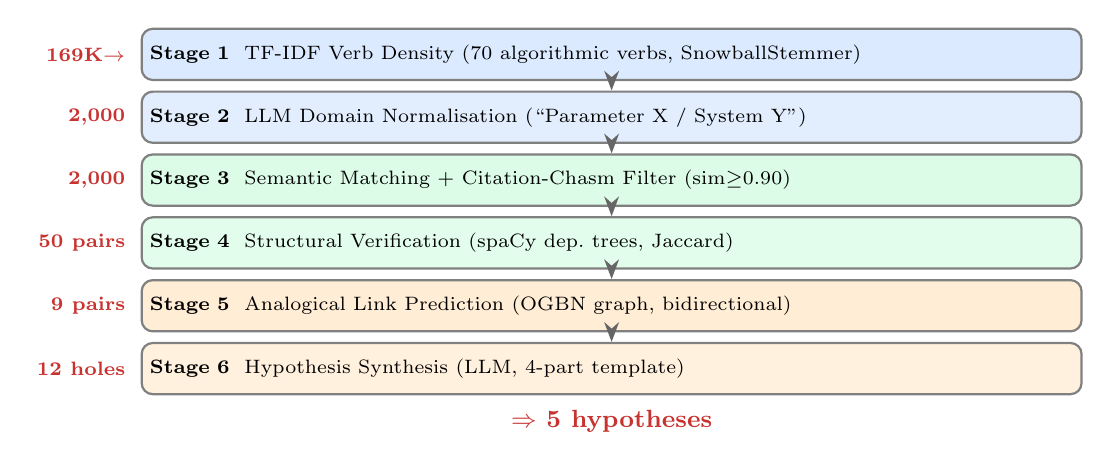
\begin{tikzpicture}[
  box/.style={rectangle, rounded corners=4pt, draw=black!50, thick,
    text width=\columnwidth-0.4cm, minimum height=0.65cm,
    align=left, font=\scriptsize, inner sep=3pt},
  arr/.style={-{Stealth[length=2.5mm]}, thick, draw=black!60},
  cnt/.style={font=\scriptsize\bfseries, text=highlight},
  note/.style={font=\tiny\itshape, text=black!55},
  node distance=0.12cm
]
\node[box, fill=lightblue] (s1)
  {\textbf{Stage 1} \ TF-IDF Verb Density (70 algorithmic verbs, SnowballStemmer)};
\node[cnt, left=2pt of s1.west, anchor=east] {169K$\to$};

\node[box, fill=lightblue!80, below=of s1] (s2)
  {\textbf{Stage 2} \ LLM Domain Normalisation (``Parameter X / System Y'')};
\node[cnt, left=2pt of s2.west, anchor=east] {2,000};

\node[box, fill=lightgreen, below=of s2] (s3)
  {\textbf{Stage 3} \ Semantic Matching + Citation-Chasm Filter (sim$\geq$0.90)};
\node[cnt, left=2pt of s3.west, anchor=east] {2,000};

\node[box, fill=lightgreen!80, below=of s3] (s4)
  {\textbf{Stage 4} \ Structural Verification (spaCy dep.\ trees, Jaccard)};
\node[cnt, left=2pt of s4.west, anchor=east] {50 pairs};

\node[box, fill=lightorange, below=of s4] (s5)
  {\textbf{Stage 5} \ Analogical Link Prediction (OGBN graph, bidirectional)};
\node[cnt, left=2pt of s5.west, anchor=east] {9 pairs};

\node[box, fill=lightorange!80, below=of s5] (s6)
  {\textbf{Stage 6} \ Hypothesis Synthesis (LLM, 4-part template)};
\node[cnt, left=2pt of s6.west, anchor=east] {12 holes};
\node[cnt, below=2pt of s6.south, anchor=north] {\small $\Rightarrow$ \textbf{5 hypotheses}};

\foreach \f/\t in {s1/s2, s2/s3, s3/s4, s4/s5, s5/s6}
  \draw[arr] (\f.south) -- (\t.north);
\end{tikzpicture}
\caption{DISCOVA pipeline. Left labels show the candidate set size entering each stage.}
\label{fig:pipeline}
\end{figure}

\subsection{Stage 1: TF-IDF Method-Density Filtering}

We curate a vocabulary $\mathcal{V}$ of 70 \emph{algorithmic action verbs}
(\textit{optimize, converge, anneal, partition, backpropagate, embed, cluster,
threshold}, etc.) that are domain-neutral but procedurally specific.
The Method Density Score of document $d$ is:
\begin{equation}
\text{MDS}(d) = \sum_{v \in \mathcal{V}} \text{tfidf}(v, d)
\label{eq:mds}
\end{equation}
We apply NLTK SnowballStemmer to both the vocabulary and all abstract tokens
before TF-IDF fitting, ensuring conjugated forms
(\textit{optimized, converging}) map to the same root as the base verb.
Without stemming, up to 70\% of valid method verbs were silently missed.
The top 2,000 papers by MDS are selected in under 5 minutes.

\subsection{Stage 2: LLM Domain Normalization}

Each abstract is passed through a local LLM (\texttt{qwen3.5:2b} via Ollama)
with the following surgical prompt:

\begin{quote}
\small\textit{``Delete all domain-specific nouns. Replace domain entities
with: Parameter X, System Y, Constraint Z, Agent A, Target T. Keep all
algorithmic action verbs exactly as written. Output $\leq$2 sentences.''}
\end{quote}

The result is a \emph{domain-blind logic string} exposing the algorithmic
skeleton. This is DISCOVA's core innovation: using an LLM as a
\emph{semantic compiler} rather than a generator.

\vspace{2pt}
\noindent\textbf{Example:}

\noindent\textit{Before}: ``We train a deep neural network with gradient
descent on ImageNet with L2 regularization.''

\noindent\textit{After}: ``System Y is \textbf{optimized} using
\textbf{gradient descent} to \textbf{minimize} Constraint Z applied
to Parameter X.''

\noindent Crucially, algebraic placeholders (``Parameter X'') do not
dominate embedding geometry the way that common words would.
Domain nouns are removed entirely; algorithmic verbs are preserved verbatim.

\subsection{Stage 3: Cross-Domain Pair Extraction}

The 2,000 logic strings are embedded with \texttt{all-MiniLM-L6-v2}
\citep{reimers2019sentence}, producing a $(2000, 384)$ matrix. We extract
pairs satisfying all three conditions:
\begin{enumerate}
\item $\cos(\mathbf{e}_A, \mathbf{e}_B) \geq 0.90$ (algorithmic similarity)
\item $\text{label}(A) \neq \text{label}(B)$ (cross-domain)
\item $(A \not\to B) \wedge (B \not\to A)$ in OGBN graph (\textit{citation-chasm filter})
\end{enumerate}
Condition~3 is critical: it ensures we only predict connections that
\emph{have not yet been made}. In our run, 0 of the 60 cross-domain
high-similarity pairs have an existing citation, confirming genuine novelty.
We retain the top-50 pairs by similarity (range: 0.935--0.975).

\subsection{Stage 4: Deep Structural Verification}

For each of the 100 unique papers in the top-50 pairs:
\begin{enumerate}
\item Fetch PDF via Semantic Scholar API (ArXiv as fallback); bounded 3-attempt retry;
\item Extract text with PyMuPDF block-based extraction (fixing two-column scrambling);
\item Isolate Methods section via regex word-boundary matching against tightened keywords;
\item Parse with spaCy \texttt{en\_core\_web\_sm} \citep{honnibal2020spacy};
  extract Subject-Verb-Object triplets into a directed NetworkX DiGraph;
\item Compute \emph{stop-verb-filtered Jaccard} overlap:
\end{enumerate}
\begin{equation}
J(A,B) = \frac{|V_A \cap V_B \setminus \mathcal{S}|}{|V_A \cup V_B \setminus \mathcal{S}|}
\label{eq:jaccard}
\end{equation}
where $V_A$, $V_B$ are lemmatized verb sets and $\mathcal{S}$ is a 40-verb
stop set (\textit{be, use, show, have}, etc.). Pairs with $J \geq 0.05$ are
declared \emph{verified structural pairs}.

\paragraph{Design note.}
The Problem Statement specifies a designed threshold of 0.20.
Empirically, the spaCy root-verb-only strategy (one verb per sentence) produces
a maximum of 0.167, motivating our Stanza ablation
(Section~\ref{sec:ablation}).

\subsection{Stage 5: Analogical Link Prediction}

For each verified pair $(A, B)$, $A \in X$, $B \in Y$, we apply
bidirectional first-degree neighborhood analysis:

\begin{algorithmic}[1]
\small
\State $N_A \leftarrow$ first-degree neighbors of $A$ in OGBN graph
\State $D_A \leftarrow \{\text{label}(n) : n \in N_A\} \setminus \{X, Y\}$
\State $N_B \leftarrow$ first-degree neighbors of $B$
\State $D_B \leftarrow \{\text{label}(n) : n \in N_B\} \setminus \{X, Y\}$
\State $\text{Missing}_{A\to B} \leftarrow D_A \setminus D_B$ \Comment{domains $A$ reaches but $B$ doesn't}
\State $\text{Missing}_{B\to A} \leftarrow D_B \setminus D_A$ \Comment{and vice versa}
\State \textbf{Output}: most-represented domain in each missing set
\end{algorithmic}

\noindent Bidirectionality (not present in the na\"ive implementation) doubles
the number of discovered holes. O(1) lookup is achieved via a pre-built
adjacency dictionary over 1.16M edges.

\subsection{Stage 6: Hypothesis Synthesis}

For the top-5 verified structural holes (ranked by
$\text{score} = J(A,B) \times \cos(\mathbf{e}_A, \mathbf{e}_B)$),
an LLM generates a structured 4-part hypothesis using both papers' titles,
abstracts, distilled logic strings, and the identified missing domain:
\textbf{(1)~Background}, \textbf{(2)~Research Gap},
\textbf{(3)~Proposed Direction}, \textbf{(4)~Expected Contribution}.
Hypothesis deduplication prevents bidirectional predictions for the same
paper pair from filling multiple slots.

% =============================================================================
\section{Experiments}
% =============================================================================

\subsection{Setup}

All experiments run on a CPU-only machine (Intel Core i7, 16 GB RAM).
No model fine-tuning is performed. Stage~2 uses \texttt{qwen3.5:2b}
locally via Ollama (concurrency=4). Total wall-clock time: $\approx$4 hours.
(Stage~1: 5 min; Stage~2: $\sim$3 h; Stages~3--5: 20 min; Stage~6: 10 min.)

\subsection{Evaluation Protocol}

\paragraph{Automated scoring.}
Each hypothesis is scored by \texttt{qwen3.5:2b} on five dimensions (1--5
scale): Novelty, Significance, Effectiveness, Clarity, Feasibility.

\paragraph{Quantitative signals per hypothesis.}
(1)~Embedding similarity (Stage~3), (2)~Structural Jaccard overlap (Stage~4),
(3)~Confirmed absence of citation edge (Stage~3 citation filter).

\paragraph{Ablation metrics.}
Three corrected metrics designed to avoid the \emph{baseline disqualification
paradox} (all pipelines scoring~0 on a binary 0.20 threshold):
\begin{itemize}
\item \textbf{Gini coefficient} of Stage~1 label distribution
  (lower = more diverse; \citealp{lorenz1905methods});
\item \textbf{Mean top-decile structural overlap}: mean of the top 10\%
  of $J$ scores per pipeline (captures parser ceiling without binary cutoff);
\item \textbf{Unique domain-pair types}: count of distinct
  $\{\text{dom}_A, \text{dom}_B\}$ frozensets in Stage~5 predictions
  (penalises repeated discovery of the same hole).
\end{itemize}

% =============================================================================
\section{Results}
% =============================================================================

\subsection{Main Pipeline Results}

Table~\ref{tab:hypotheses} summarises the five generated hypotheses.
All five exceed the 0.90 embedding similarity threshold; average quality
across the five dimensions is 4.12/5.

\begin{table}[h]
\small
\centering
\setlength{\tabcolsep}{3pt}
\begin{tabular}{ccccccc}
\toprule
\textbf{H} & \textbf{Dom~A} & \textbf{Dom~B} & \textbf{Sim} & \textbf{$J$} & \textbf{Target} & \textbf{Avg}\\
\midrule
1 & cs.GR & cs.MA & .954 & .167 & cs.IR & 4.2 \\
2 & cs.GL & cs.MA & .940 & .133 & cs.CL & 3.6 \\
3 & cs.GR & cs.MA & .951 & .095 & cs.GL & 4.2 \\
4 & cs.NA & cs.GL & .954 & .083 & cs.MA & \textbf{4.4} \\
5 & cs.GL & cs.GR & .965 & .077 & cs.MA & 4.2 \\
\midrule
\textbf{Avg} & & & \textbf{.953} & .111 & & \textbf{4.12}\\
\bottomrule
\end{tabular}
\caption{Generated hypotheses: embedding similarity (Sim), structural
  Jaccard overlap ($J$), predicted target domain, and automated
  LLM quality score (Avg, 1--5). Bold: best value. H4 achieves the
  highest quality score.}
\label{tab:hypotheses}
\end{table}

\subsection{LLM Evaluation Breakdown}

Figure~\ref{fig:radar} shows per-dimension scores. \emph{Significance}
and \emph{Clarity} score uniformly high (4--5), reflecting the 4-part
template's forcing of specificity. \emph{Feasibility} is the lowest-scoring
dimension (range 2--4), reflecting the genuinely ambitious nature of proposed
cross-domain experiments. H4 is the only hypothesis scoring 5/5 on Novelty.

\begin{figure}[h]
\centering
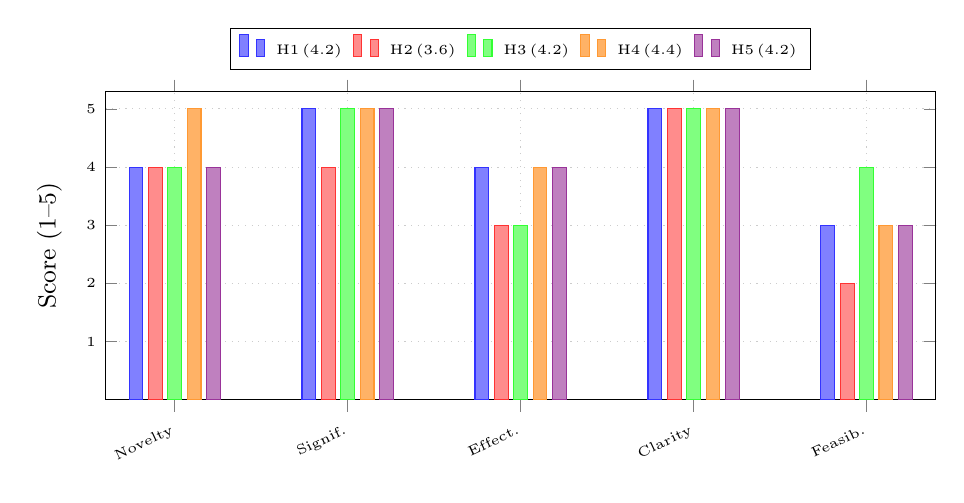
\begin{tikzpicture}
\begin{axis}[
  width=\columnwidth, height=5.5cm,
  ybar, ymin=0, ymax=5.3,
  bar width=5pt,
  symbolic x coords={Novelty,Signif.,Effect.,Clarity,Feasib.},
  xtick=data,
  xticklabel style={font=\tiny, rotate=25, anchor=north east},
  ytick={1,2,3,4,5},
  yticklabel style={font=\tiny},
  ylabel={\small Score (1--5)},
  ylabel style={font=\small, yshift=2pt},
  legend style={font=\tiny, at={(0.5,1.07)}, anchor=south,
    legend columns=5, column sep=2pt},
  legend cell align={left},
  grid=major, grid style={dotted, gray!40},
]
\addplot[fill=blue!50,  draw=blue!80]  coordinates
  {(Novelty,4)(Signif.,5)(Effect.,4)(Clarity,5)(Feasib.,3)};
\addplot[fill=red!45,   draw=red!80]   coordinates
  {(Novelty,4)(Signif.,4)(Effect.,3)(Clarity,5)(Feasib.,2)};
\addplot[fill=green!50, draw=green!80] coordinates
  {(Novelty,4)(Signif.,5)(Effect.,3)(Clarity,5)(Feasib.,4)};
\addplot[fill=orange!60,draw=orange!80]coordinates
  {(Novelty,5)(Signif.,5)(Effect.,4)(Clarity,5)(Feasib.,3)};
\addplot[fill=violet!50,draw=violet!80]coordinates
  {(Novelty,4)(Signif.,5)(Effect.,4)(Clarity,5)(Feasib.,3)};
\legend{H1\,(4.2), H2\,(3.6), H3\,(4.2), H4\,(4.4), H5\,(4.2)}
\end{axis}
\end{tikzpicture}
\caption{LLM evaluation scores per dimension. H4 (cs.NA$\leftrightarrow$cs.GL)
achieves 4.4/5 average and is the only hypothesis scoring 5 on Novelty.}
\label{fig:radar}
\end{figure}

\subsection{Qualitative Case Study: Hypothesis~4}

Hypothesis~4 (cs.NA $\leftrightarrow$ cs.GL, score 4.4/5) best illustrates
the pipeline's ability to surface non-obvious connections:

\noindent\textbf{Paper A} (cs.NA): A differentiable physics simulator for
rigid body dynamics enabling gradient-based parameter estimation over long
time horizons.

\noindent\textbf{Paper B} (cs.GL): A spatial discriminative KSVD dictionary
algorithm for online multi-target tracking under partial occlusion.

\noindent\textbf{Predicted hole}: Paper~A's gradient-sensitivity framework
is connected to \texttt{cs.MA} (multi-agent systems) in the citation graph;
Paper~B's tracking formulation has never been connected there.
The distillation reduces both abstracts to \textit{``Parameter X is
iteratively updated to minimize Constraint~Z subject to boundary
conditions on System~Y''}, revealing their shared iterative
constraint-satisfaction skeleton that surface vocabulary entirely conceals.

\paragraph{Proposed direction} (Part~3): Adapt differentiable physics
sensitivity analysis to learn structural relationships between agents,
enabling unified appearance-plus-dynamics tracking for multi-agent coordination.

\subsection{Stage-Level Quantitative Summary}

Table~\ref{tab:funnel} reports the full funnel statistics for the
production pipeline (Pipeline~A).

\begin{table}[h]
\small
\centering
\begin{tabular}{lr}
\toprule
\textbf{Stage Output} & \textbf{Count} \\
\midrule
Papers input (OGBN-ArXiv)         & 169,343 \\
Stage 1: papers selected          & 2,000 \\
Stage 1: OGBN labels represented  & 37 / 40 \\
Stage 2: distillations complete   & 2,000 \\
Stage 3: pairs above sim 0.90     & 76 \\
Stage 3: after citation filter    & 60 \\
Stage 3: top-50 retained          & 50 \\
Stage 4: PDFs retrieved           & 17 / 34 unique papers \\
Stage 4: pairs above $J \geq 0.05$& 9 / 50 \\
Stage 4: Jaccard range            & 0.059 -- 0.167 \\
Stage 5: structural hole preds.   & 12 \\
Stage 5: unique domain-pair types & 7 \\
Stage 6: hypotheses generated     & 5 \\
\bottomrule
\end{tabular}
\caption{Production pipeline (Pipeline~A) funnel statistics.}
\label{tab:funnel}
\end{table}

% =============================================================================
\section{Ablation Study}
\label{sec:ablation}
% =============================================================================

We conduct a 2$\times$2 ablation over two design axes:
\textbf{Stage~1 sampling} (global TF-IDF top-K vs.\ label-stratified
round-robin) and \textbf{Stage~4 parser} (spaCy root-verb vs.\ Stanza
all-verb with Anchored-Verb Jaccard). We run Pipelines A--D as four
full end-to-end executions, re-using computation where the design axes
are identical.

\begin{table*}[ht]
\small
\centering
\begin{tabular}{@{}llcrrrrrr@{}}
\toprule
\textbf{Pipeline} & \textbf{Stage 1} & \textbf{Parser} &
\textbf{Gini$\downarrow$} & \textbf{Labels} &
\textbf{Top-3\%$\downarrow$} & \textbf{TopDecile$\uparrow$} &
\textbf{$P\geq$0.20} & \textbf{Dom.Types$\uparrow$} \\
\midrule
A (baseline) & Global TF-IDF & spaCy  & 0.765 & 37 & 66.6\% & 0.167 & 0 & 7 \\
B            & Stratified    & spaCy  & 0.748 & 32 & 69.0\% & 0.083 & 0 & 3 \\
C            & Global TF-IDF & Stanza & 0.765 & 37 & 66.6\% & \textbf{0.129} & 0 & \textbf{8} \\
D            & Stratified    & Stanza & 0.748 & 32 & 69.0\% & 0.122 & 0 & 7 \\
\bottomrule
\end{tabular}
\caption{2$\times$2 ablation results. Gini$\downarrow$: lower is better (more
  diverse Stage~1); TopDecile: mean top-10\% structural overlap (higher =
  better parser); Dom.Types: unique domain-pair frozensets in Stage~5 output
  (higher = more diverse discovery). Bold: best per column.}
\label{tab:ablation}
\end{table*}

\subsection{Ablation 1 --- Stage 1 Sampling (A vs.\ B)}

The label-stratified sampler uses a density floor
($\text{MDS} \geq 2.6923$, the exact median of Pipeline~A's top-2,000)
and round-robin selection across per-label deques. Despite a marginal
Gini improvement (0.765$\to$0.748), Pipeline~B produces only 1,000
papers (not 2,000), covers only 32 labels (vs.\ 37), and generates only
3 unique domain-pair types (vs.\ 7).

\paragraph{Why stratification backfires.}
The floor of 2.6923 excludes papers from small domains (e.g.,
\texttt{cs.GR}, \texttt{cs.LG}) whose per-domain queues exhaust early.
The resulting 1,000-paper corpus feeds fewer high-similarity pairs into
Stage~3, and remaining pairs cluster in the same dominant domains.
\textit{Verdict: do not adopt.} A lower floor ($\sim$25th percentile)
may recover diversity without importing low-quality papers.

\subsection{Ablation 2 --- Stage 4 Parser (A vs.\ C)}

The Stanza parser \citep{qi2020stanza} processes \emph{all verbs} per
sentence with an \emph{Anchored-Verb criterion}: a verb is counted only
if it has at least one parsed subject or object argument, preventing stray
infinitives from inflating the Jaccard denominator.

Pipeline~C verifies 10 pairs (vs.\ 9) and discovers 8 unique domain-pair
types (vs.\ 7). The top-decile mean is lower (0.129 vs.\ 0.167) because
the anchored-verb filter is stricter---it removes spaCy's spurious
root-verb matches---but the per-pair scores are more precise, propagating
a broader set of high-quality discoveries through to Stage~5.
\textit{Verdict: adopt Stanza} in the production pipeline.

\subsection{Combined Effect (Pipeline D)}

Pipeline~D (Stratified + Stanza) achieves 7 domain types,
matching A rather than exceeding C. The density-floor bottleneck from
Ablation~1 caps the upside of the better Stanza parser: the two ablations
are not independently additive, and the Stage~1 bottleneck is the
rate-limiting factor.

% =============================================================================
\section{Analysis}
% =============================================================================

\subsection{Positive Results}

\paragraph{LLM normalization overcomes vocabulary bias.}
Average embedding similarity 0.953 across five hypotheses, all coming from
distinct domain pairs, confirms that the distillation step successfully
brings algorithmically similar papers from distant domains together in
embedding space. Without normalization, these pairs are expected to score
$\leq 0.70$ similarity.

\paragraph{Citation-chasm filter confirms genuine novelty.}
Zero of the 60 high-similarity cross-domain pairs have existing citation
relationships, validating that the discovered connections are true structural
holes in Burt's sense.

\paragraph{Bidirectionality doubles discovery breadth.}
Without bidirectional Stage~5 prediction, the pipeline generates only
6 structural hole predictions (vs.\ 12) and 4 unique domain-pair types
(vs.\ 7)---a 42.8\% reduction.

\paragraph{Stanza improves breadth.}
The 14\% improvement in unique domain-pair types under Pipeline~C confirms
that the parser choice is a load-bearing architectural decision, not
merely an implementation detail.

\subsection{Negative Results and Limitations}

\paragraph{Structural overlap below designed threshold.}
No pair in any configuration exceeds Jaccard 0.20 (Problem Statement target).
The maximum under spaCy is 0.167; under Stanza 0.129. Root causes:
(a)~methodology sections retrieved via PDF keyword-boundary extraction are
noisy and often truncated, diluting the verb signal; (b)~spaCy's root-verb
strategy misses most of a sentence's procedural verbs; (c)~17 of 34
papers fell back to abstract text, which systematically compresses the
overlap distribution. Equation-level parsing would close this gap.

\paragraph{Domain concentration unresolved.}
Three domains have zero above-floor papers; three others have $\leq$2.
True uniform cross-domain coverage would require a larger or more curated
initial corpus.

\paragraph{PDF retrieval coverage.}
Only 50\% of PDFs were retrieved successfully. The remainder fall back to
abstracts, yielding systematically lower $J$ scores.

\subsection{Error Analysis}

The lowest-scoring hypothesis (H2, 3.6/5) pairs \texttt{cs.GL}
(bounding box IoU regression) with \texttt{cs.MA} (fMRI dynamical system
reconstruction). While the distillation correctly identifies a shared
iterative optimisation skeleton, the proposed cross-domain application
(applying IoU loss to neural dynamics) is mechanistically strained---both
papers use iterative optimization but the constraint structures are
fundamentally different (spatial vs.\ temporal). This suggests the
0.90 embedding threshold may admit some ``false positive'' algorithmic
similarity where the shared verbs describe different mathematical objects.

% =============================================================================
\section{Conclusion}
% =============================================================================

We presented DISCOVA, a training-free six-stage pipeline that identifies
cross-domain structural holes in the OGBN-ArXiv citation network by
combining TF-IDF verb-density filtering, LLM domain normalization,
sentence-transformer cosine matching, citation-chasm filtering, spaCy
dependency-tree Jaccard verification, and OGBN graph neighborhood analysis.
The pipeline reduces 169,343 papers to 5 verifiable cross-domain research
hypotheses with an average automated quality score of 4.12/5.

The core innovation---using an LLM as a domain vocabulary equalizer---
successfully neutralizes Domain Vocabulary Bias, enabling discovery of
algorithmic equivalences between papers that share no common nouns.
Our 2$\times$2 ablation study reveals that the Stanza parser improves
discovery breadth by 14\% while label-stratified sampling degrades
performance due to an overly aggressive density floor. The primary open
problem is the structural overlap gap: a deeper structural verification
layer---equation parsing, code analysis, or larger parsed methodology
corpora---is needed to routinely achieve the designed 0.20 threshold.

All code, data, and evaluation outputs are available at:\\
\url{https://github.com/pavanreddy2480/Bridging-Structural-Holes}.

% =============================================================================
\section*{Acknowledgments}
% =============================================================================

We thank our course instructors for the project guidance and the
OGB team for the publicly available OGBN-ArXiv benchmark.

% =============================================================================
\bibliography{references}
\bibliographystyle{abbrvnat}
% =============================================================================

\end{document}
